\documentclass{tufte-handout}

\title{Road safety's Vision Zero: applications to OH\&S}

\author{Dr James Reynolds, Public Transport Research Group}

%\date{28 March 2010} % without \date command, current date is supplied

%\geometry{showframe} % display margins for debugging page layout

\usepackage{graphicx} % allow embedded images
  \setkeys{Gin}{width=\linewidth,totalheight=\textheight,keepaspectratio}
  \graphicspath{{graphics/}} % set of paths to search for images
\usepackage{amsmath}  % extended mathematics
\usepackage{booktabs} % book-quality tables
\usepackage{units}    % non-stacked fractions and better unit spacing
\usepackage{multicol} % multiple column layout facilities
\usepackage{lipsum}   % filler text
\usepackage{fancyvrb} % extended verbatim environments
\usepackage{pgfplots}
  \fvset{fontsize=\normalsize}% default font size for fancy-verbatim environments

% Standardize command font styles and environments
\newcommand{\doccmd}[1]{\texttt{\textbackslash#1}}% command name -- adds backslash automatically
\newcommand{\docopt}[1]{\ensuremath{\langle}\textrm{\textit{#1}}\ensuremath{\rangle}}% optional command argument
\newcommand{\docarg}[1]{\textrm{\textit{#1}}}% (required) command argument
\newcommand{\docenv}[1]{\textsf{#1}}% environment name
\newcommand{\docpkg}[1]{\texttt{#1}}% package name
\newcommand{\doccls}[1]{\texttt{#1}}% document class name
\newcommand{\docclsopt}[1]{\texttt{#1}}% document class option name
\newenvironment{docspec}{\begin{quote}\noindent}{\end{quote}}% command specification environment

\begin{document}

\maketitle% this prints the handout title, author, and date

\begin{abstract}
\noindent
Road safety engineering in Australia has a long history of improvements in practice leading to reductions in the rate of fatal and serious injury crash outcomes.  Researchers across Monash, including from Civil Engineering and the Accident Research Centre (MUARC), have been involved in moving, and helped lead, the science and public conversation closer 'Towards Zero'. This includes advocating for wider adoption of the Safe System approach, in which there is an acknowledgement that human error is inevitable, and that it is road designers and managers, rather than users, who have primary responsibility for ensuring safe outcomes. Underlying this is 'Vision Zero': a position that death or serious injury should never be the outcome of failures\cite{Lydon:2017aa}.

Are our current  approaches to (non-road-related) OH\&S matters aligned with the Safe System philosophy? What differences are there between our current risk-management assessments (based on reducing likely and/or severity) and a 'Vision-Zero-informed'  approach to eliminating death and serious injury outcomes entirely? This Safety Day discussion explores these issues, and provides perspectives from road safety engineering, where death and serious injury remains a daily occurence, on how (non-transport-related) safety management might be further improved.\end{abstract}

%A Road Safety Audit (RSA) is a formal process used in traffic engineering to assess the crash potential of new and existing facilities. The aim is to identify potentially hazardous conditions and recommendations.  It is often used during design or immediately after construction is complete so that unsafe features can be identified and corrected  \textbf{before} anyone uses the road. 


\begin{marginfigure}
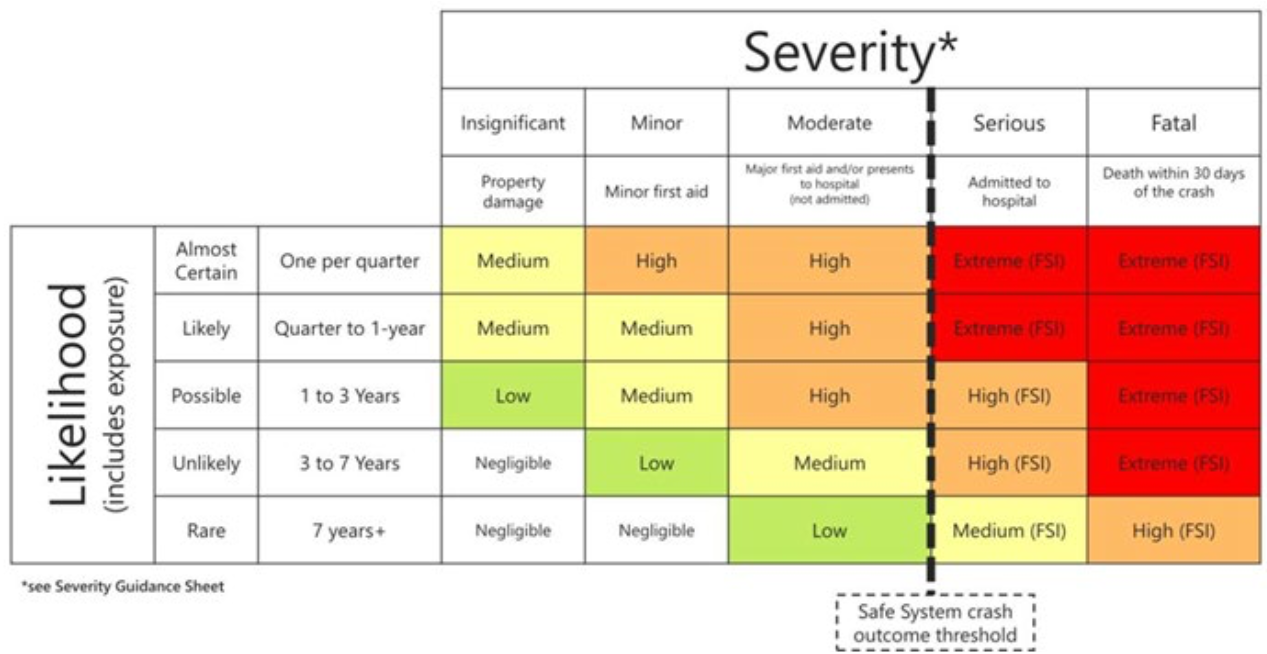
\includegraphics{Austroads_risk_matrix}
\caption{Austroads Road Safety Audit risk matrix}
\label{fig:Austroads_risk_matrix}
\end{marginfigure}


The most recent Guide to Road Safety Auditing\cite{Hillier:2022aa} includes a new risk assessment matrix (Figure \ref{fig:Austroads_risk_matrix}). It is similar to most, with likelihood and severity combined to given a ranking of risk from negligible (white) to extreme (red). What is different, however, is the large black line separating 'moderate' crashes resulting in injury and presentation to hospital, from 'serious' crashes resulting in hospital admission and 'fatal' crashes (Figure \ref{fig:Austroads_risk_matrix_excerpt}).  

\begin{marginfigure}
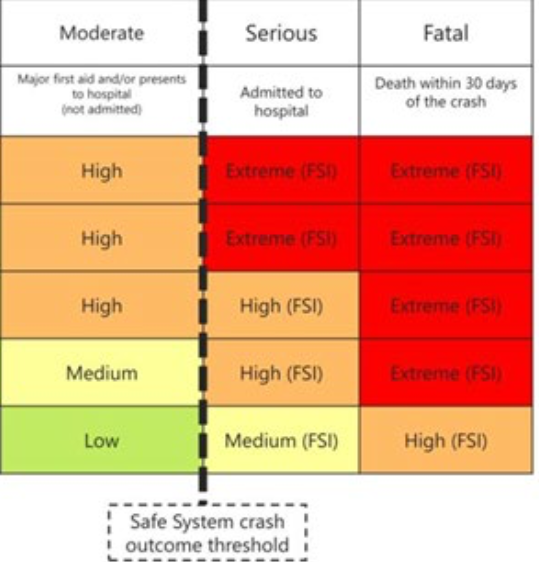
\includegraphics{Austroads_risk_matrix_excerpt}
\caption{Austroads Road Safety Audit risk matrix - Moderate, Serious and Fatal}
\label{fig:Austroads_risk_matrix_excerpt}
\end{marginfigure}

This represents the threshold between crashes that result in fatality or serious injury (FSI) and those that do not. Under the Safe System and Vision Zero such crash outcomes are \textbf{never} considered acceptable.  It is \textbf{not} sufficient to reduce the likelihood. Rather, these problems must be treated in a way that reduces the severity of outcomes below the threshold.   

This has resulted in a change to the way that us Road Safety Auditors make findings and recommendations. The problem with recommending measures that only reduce likelihood\footnote{e.g. linemarking, tactile pavement markers or better lighting.} is that they \textbf{do not eliminate} the possibility of serious injury or fatality. Such measures still have their place, but no matter how much linemarking or shoulder sealing is installed, when considering the amount of driving done across the population, at some stage someone is going to depart the traffic lane and impact something at speed that might result in death.  

This is part of the reason that wire rope safety barrier, lower speed limits and other such measures that lower crash severity are now often recommended in Road Safety Audits, and installed along roads. An impact speed of around 70km/hr is the typical threshold for head-on crashes to result in serious injury or fatality\footnote{50km/hr for right angle crashes, 40km/hr for impact with roadside object, 30km/hr for crash involving pedestrian, cyclist or motorcyclist (see Hillier (2022) cited above). That said, a (1-2 ton) car can crush you even moving at low speeds.} and so it is now common to see wire rope safety barrier in the centre of highways or freeway medians.  Wire rope safety barrier will not reduce the likelihood of an errant vehicle, but it will prevent that vehicle from hitting someone coming in the opposite direction, and keep impact forces within the tolerance of a human body\cite{TAC:2016aa}.  

\begin{marginfigure}
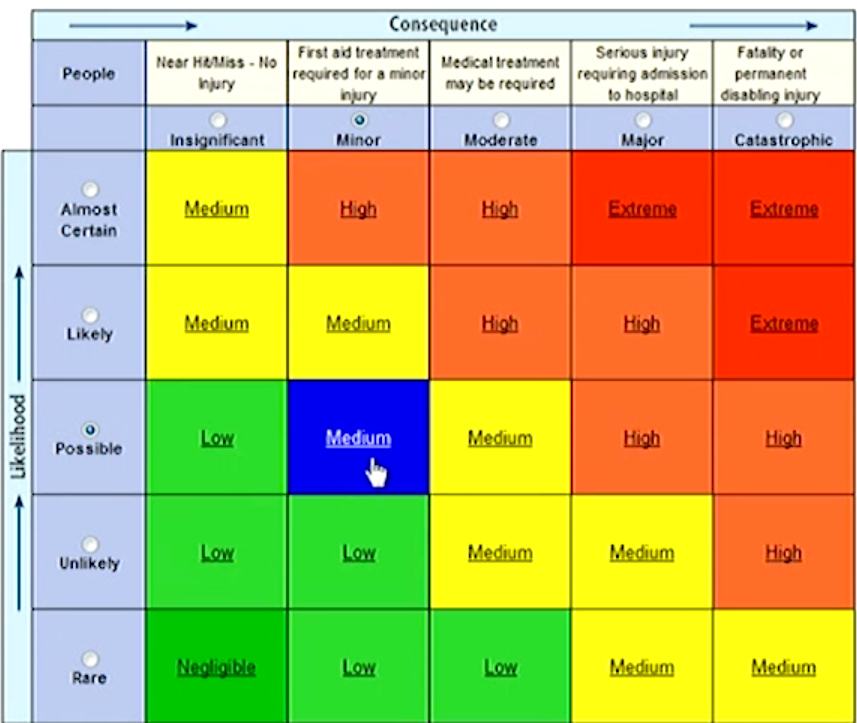
\includegraphics{SARAH_risk_matrix}
\caption{Risk matrix, SARAH}
\label{fig:SARAH}
\end{marginfigure}

\newthought{So what do we do in OH\&S management?} Figure \ref{fig:SARAH} shows the risk matrix used in the SARAH system here at Monash.  The highlighted location is a 'medium' risk, at the intersection of a 'probable' event that results in 'minor' injury (resulting in a need for first aid).  This 'medium' risk level is \textbf{identical} to that for an 'unlikely' event resulting in hospital admission, or a 'rare' event resulting in fatality or permanent disabling injury. In contrast, under a 'Vision Zero' approach, the hospital admission or fatal outcome incidents would be separately categorised, identifying the need to reduce consequences to less than the FSI threshold or otherwise eliminate the hazard. 

%\begin{marginfigure}
%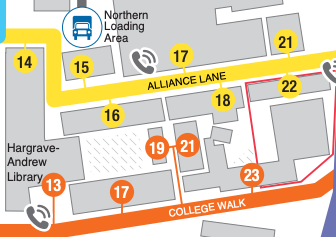
\includegraphics{Clayton_map_excerpt}
%\caption{Alliance Lane and surrounds, Clayton campus}
%\label{fig:Alliance_lane}
%\end{marginfigure}


\begin{marginfigure}
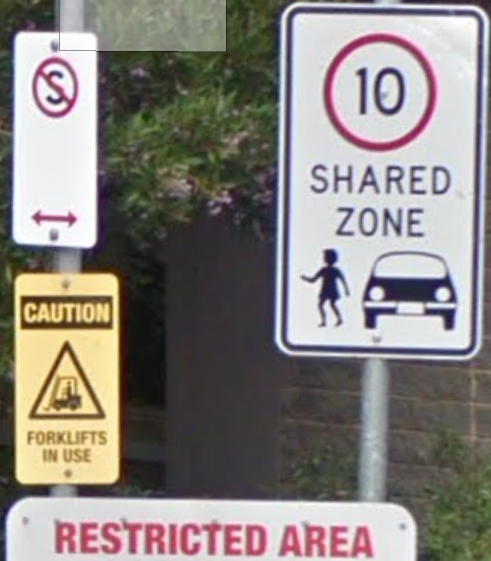
\includegraphics{Alliance_lane_forklifts}
\caption{Alliance Lane warning sign}
\label{fig:Alliance_lane_forklifts}
\end{marginfigure}


Thinking of a practical example from Clayton, there is a warning sign in Alliance Lane about forklifts being in use (Figure \ref{fig:Alliance_lane_forklifts}) within a shared zone. The purpose of this sign appears to be to reduce the likelihood that a pedestrian and forklift collide, by warning pedestrians to be vigilant. However, both are apparently allowed to be in the same place at the same time, meaning that a pedestrian being crushed to death by a forklift is still a possible outcome\footnote{Think of a child that gets away, a student distracted by stress, or someone who does not see or ignores the sign.}, even though this would be an incredibly rare event. Contrast this to the warehouse space immediately before the checkouts at any IKEA. This is used by both shoppers and forklifts, but never at the same time. 


\newthought{In summary} the key message from road safety engineering is to focus especially on hazards that might causes serious injury or fatality (no matter how unlikely). Reducing consequences or total elimination of these is at the core of the new(-ish) Vision-Zero-based thinking in road safety engineering, although there is clearly a long way to go\footnote{241 road deaths in Victoria in 2022 (Source: https://www.tac.vic.gov.au/)}. While the context in OH\&S is different\footnote{66 workplace deaths in Victoria in 2022 (Source: https://www.worksafe.vic.gov.au)} the Safe System approach would imply the use of measures that reduce the severity of potentially fatal or serious injury outcome incidents (or make these entirely impossible). In road safety we are shifting to acknowledge that human error is inevitable, and that systems need to fail safely. I recommend doing the same in you management of OH\&S risks.


%\printclassoptions

\nobibliography{safety_day_2023_handout}
\bibliographystyle{plainnat}



\end{document}
